
\section{Visualization ideas}

  \begin{frame}
    \frametitle{General ideas}
    
    General ideas so far \red{feel free to propose whatever else, pretty please!!!)}: 
    ~\\~\\
       
    zoomable map with aggregated data about all attacks per country and more details when zoomed-in
    \begin{itemize}
        \item facets: time(range); checkboxes for types of targets / weapons / attacks; maybe also group;
        \item maybe size of 'point' or color of country per \#attacks or per \#victims/\# wounded (or per whatever else)
        \item turn on/off flow map for where attackers come from (into each country)
        \item The "Small Multiple Circle Packing" stuffs might be used for types of w/a/t/g in the main view
    \end{itemize}

  \end{frame}


  \begin{frame}
    \frametitle{General ideas}

    click on country $\rightarrow$ data about all attacks in the country; 
    \begin{itemize}
        \item Maybe timeline
        \item wordcloud with motives for attacks
        \item Maybe something like "A circular flow diagram (Sankey meets Chord diagram)" or "Re-usable Sankey" for types of weapons/attacks/targets/groups
        \item Sth like a star chart to compare \#attacks/victims/etc per group in a country     
    \end{itemize}

  \end{frame}
  
  \begin{frame}
    \frametitle{General ideas}

    click on attach $\rightarrow$ simply visualize everything about this attack (with all text around, a bit of a 'story telling' part)
    \begin{itemize}
        \item Maybe just a pretty but extremely sad template with nicely placed text and general info...?
    \end{itemize}


  \end{frame}



  \begin{frame}
    \frametitle{Other ideas}
    
    Other random ideas?
 
    And yes, we've seen that it's visualized already http://start.umd.edu/gtd/globe/index.html but it sucks, so ours will be way more cool

  \end{frame}



  \begin{frame}
    \frametitle{E.g. a zoomable map as a beginning}
    
    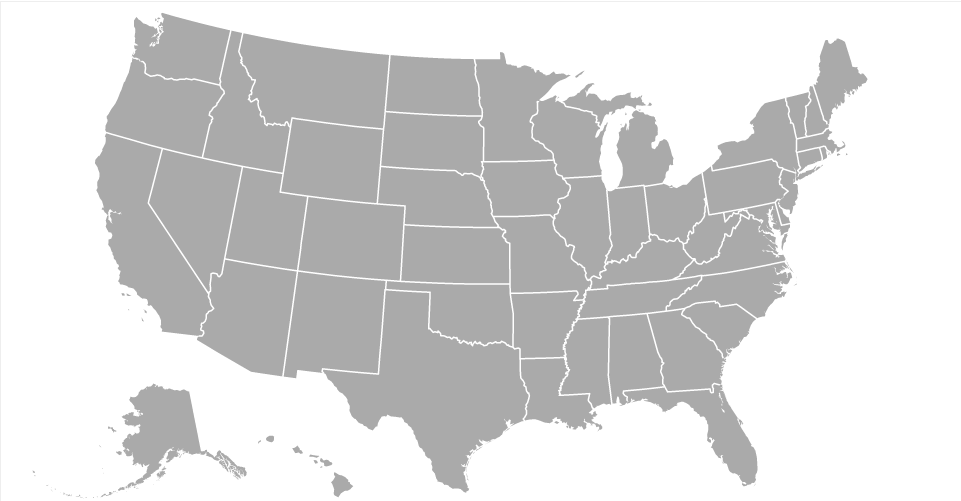
\includegraphics[width=\textwidth]{Figures/zoomable_map.png}


  \end{frame}




  \begin{frame}
    \frametitle{MAY WE PLEASE HAVE A BRAINSTORM LIKE THIS WITH OUR IDEAS!!! :D }
    
    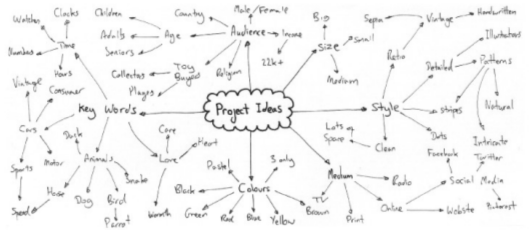
\includegraphics[width=\textwidth]{Figures/project_ideas.png}


  \end{frame}


